\chapter{Các công trình liên quan}
\ifpdf
    \graphicspath{{Chapter2/Chapter2Figs/PNG/}{Chapter2/Chapter2Figs/PDF/}{Chapter2/Chapter2Figs/}}
\else
    \graphicspath{{Chapter2/Chapter2Figs/EPS/}{Chapter2/Chapter2Figs/}}
\fi

\markboth{\MakeUppercase{Chương \thechapter. Các công trình liên quan}}{Chương \thechapter. Các công trình liên quan}

Trong chương này chúng tôi sẽ trình bày một cách tổng quan về các phương pháp truy vấn đối tượng trên tập dữ liệu ảnh lớn đang được sử dụng rộng rãi hiện nay. Các phương pháp cần phải thỏa hai yêu cầu là cho kết quả với độ chính xác cao và trả về trong thời gian gần như ngay lập tức.\\
Để có thể truy vấn hình ảnh trong thời gian ngắn, mọi dữ liệu phải được lưu trữ trên RAM vì tốc độ truy xuất ổ cứng rất chậm. Tuy nhiên do dung lượng rất hạn chế của RAM, ta phải tìm cách biểu diễn tập dữ liệu hình ảnh cho phù hợp để vừa đảm bảo được về mặt không gian lưu trữ, vừa đáp ứng được các yêu cầu của truy vấn ảnh. Mục \ref{local-features} sẽ trình bày ngắn gọn về hướng tiếp cận biểu diễn hình ảnh bằng các đặc trưng cục bộ. Nhưng khi kích cỡ của tập dữ liệu tăng thì việc so khớp các đặc trưng cục bộ tỏ ra kém hiệu quả. Trong mục \ref{bag-of-words}, chúng tôi sẽ giới thiệu mô hình Bag-of-visual-words -  được bắt nguồn từ mô hình Bag-of-Words (BoW) trong truy vấn văn bản. Mô hình này cho thấy tính hiệu quả của nó cả về tốc độ tính toán lẫn bộ nhớ sử dụng.\\
Mặc dù đạt được hiệu suất cao nhưng mô hình BoW vẫn bỏ qua thông tin về không gian ảnh - một thông tin quan trọng ảnh hướng lớn đến độ chính xác của truy vấn. Trong mục \ref{spatial}, chúng tôi sẽ trình bày rõ hơn về các hướng tiếp cận dựa để khai thác được thông tin không gian ảnh, tiêu biểu là phương pháp RASAC và Spatial Pyramid Matching (SPM).\\


\section{Biểu diễn hình ảnh bằng các đặc trưng cục bộ}
\label{local-features}

Trong lĩnh vực Thị giác Máy tính, một câu hỏi và cũng là một thách thức lớn đối với tất cả các nhà khoa học là làm sao biểu diễn được môt hình ảnh trên máy tính. Tùy theo từng mục đích cụ thể, người ta sẽ có các cách biểu diễn khác nhau. Trong truy vấn ảnh, một hình ảnh phải được biểu diễn dưới dạng sao cho bền vững trước những thay đổi như điều kiện chụp, tỉ lệ, góc chụp khác nhau hay thậm chí là những thay đổi lớn do đối tượng bị che khuất. Do sự tác động của các yếu tố này, cho dù hai hình ảnh chứa cùng một đối tượng thì vẫn có thể tồn tại một vùng hình ảnh lớn bên ngoài các đối tượng không đồng thời xuất hiện ở cả hai hình.\\
Để giải quyết vấn đề này, có một hướng tiếp cận phổ biến là rút trích những "chi tiết" cục bộ (local patches) trên tấm hình để biểu diễn cho hình ảnh đó. Hướng tiếp cận này được đưa ra dựa trên nhận định rằng hai hình ảnh tương tự nhau sẽ có rất nhiều những chi tiết cục bộ giống nhau và những chi tiết cục bộ này có thể được dùng để so khớp các hình ảnh với nhau. Các chi tiết này thường được rút trích bằng một trong hai phương pháp, đó là: (i) sử dụng một lưới dày đặc với nhiều mức tỉ lệ kích cỡ khác nhau (để đảm bảo bất biết về tỉ lệ) để chia hình ảnh thành nhiều chi tiết nhỏ, hoặc (ii) dùng các phương pháp dò tìm (detector) hay một kỹ thuật nào đó để lấy được các chi tiết đặc biệt (đặc trưng) trên vùng hình ảnh quan tâm và đồng thời loại bỏ những chi tiết không đảm bảo sự bất biến tỉ lệ ngay ở bước này. Có thể thấy rằng phương pháp dùng lưới để chia hình ảnh thành nhiều phần không thể áp dụng cho bài toán truy vấn ảnh với tập dữ liệu lớn vì ta cần rất nhiều không gian để lưu trữ một lượng lớn các chi tiết dày đặc với nhiều mức tỉ lệ kích cỡ khác nhau. Do vậy phương pháp biểu diễn hình ảnh bằng các đặc trưng được áp dụng cho bài toán này.\\
Có rất nhiều phương pháp dò tìm các đặc trưng (feature detector) được đưa ra, trong đó phải kể tới các phương pháp được dùng phổ biến như Difference of Gaussians, DoG (\cite{lowe2004distinctive}), Maximally Stable Extremal Regions, MSER (\cite{matas2004robust}) và affine invariant detector (\cite{mikolajczyk2004scale}). Ngoài ra còn có các phương pháp dò tìm được xây dựng để tìm kiếm trong thời gian thực như SURF (\cite{bay2006surf}), FAST (\cite{rosten2010faster}) và BRISK (\cite{leutenegger2011brisk}).\\
Sau khi rút trích được các đặc trưng cục bộ cho mỗi hình, dựa trên các đặc trưng đó ta sẽ quyết định xem liệu hai tấm hình bất kỳ có chứa cùng một đối tượng hay không. Để so sánh độ tương đồng của hai đặc trưng cục bộ, ta không thể dựa trên màu sắc và cường độ của chúng vì những yếu tố này không bền vững trước những thay đổi của hình ảnh. Do đó ta cần phải tìm cách lượng tử hóa độ tương đồng giữa cách đặc trưng để có thể đo được bằng các tính toán cụ thể. Trong công trình nghiên cứu nổi tiếng của \cite{lowe2004distinctive}, tác giả đã đề xuất một phương pháp để có thể tính toán được một bộ mô tả (descriptor) có tính phân loại cao và đảm bảo sự bất biến trước những thay đổi của hình ảnh, đó là SIFT descriptor. Theo sau công trình nghiên cứu này, nhiều công trình có hướng tiếp cận tương tự được đưa ra, trong đó bao gồm GLOH (\cite{mikolajczyk2005performance}), SURF (\cite{bay2006surf}), DAISY (\cite{tola2008fast}), CONGAS (\cite{zheng2009tour}), BRIEF (\cite{calonder2010brief}). Đặc biệt, bằng việc đề xuất thuật toán RootSIFT được cải tiến từ SIFT, \cite{arandjelovic2012three} đã nâng hiệu suất của phương pháp SIFT lên đáng kể. Đây cũng là phương pháp được chúng tôi chọn dùng trong hệ thống của mình.\\
Tóm lại, từ những bộ mô tả (descriptor) được rút trích từ tất cả các hình trong cơ sở dữ liệu và từ hình ảnh truy vấn, ta có thể tính toán được độ tương đồng giữa các hình ảnh. Tuy nhiên, hiệu suất của quá trình tính toán độ tương đồng bị giảm đi đáng kể khi thực hiện trên tập dữ liệu lớn. Trong phần tiếp theo, chúng tôi sẽ giới thiệu sơ lược về một mô hình giúp giải quyết được vấn đề này.

\section{Mô hình Bag-of-words}
\label{bag-of-words}
Mô hình bag-of-words đã thể hiện được sức mạnh của nó trong truy vấn văn bản và được sử dụng trong các công cụ tìm kiếm văn bản mạnh mẽ như Google, Bing. Chính vì sự thành công đó, bag-of-words đã được sử dụng trong truy vấn ảnh. Mục này chủ yếu trình bày về việc ứng dụng phương pháp truy vấn văn bản này vào trong truy vấn ảnh. Trước tiên, chúng tôi sẽ sơ lược về truy vấn văn bản, tiếp đến sẽ là việc ứng dụng của nó trong truy vấn ảnh.

\subsection{Truy vấn văn bản}
Tương tự như hình ảnh, để có thể thực hiện truy vấn với văn bản, văn bản được biểu diễn dưới dạng một mô hình không gian vector (\cite{Salton:1986:IMI:576628}) hay còn được gọi là mô hình \textit{túi từ} (bag-of-words), BoW (\cite{manning2008introduction}). Theo đó, mỗi văn bản được xem như là một tập hỗn độn (một túi) các từ và được biểu diễn dưới dạng một biểu đồ (histogram) \textit{N\textsubscript{w}}-chiều với \textit{N\textsubscript{w}} là số các từ của một ngôn ngữ. Vì giá trị của mỗi cột cột của biểu đồ bằng với số lần xuất hiện của từ tương ứng với cột đó trong văn bản nên phương pháp này còn được gọi là \textit{trọng số tần suất từ} (term frequency weighting).\\
Đôi khi, chúng ta có thể bắt gặp trường hợp nhiều từ xuất hiện trong các văn bản nhiều hơn các từ khác (ví dụ như trong tiếng Anh là \textit{the} và \textit{and}). Tuy nhiên những từ này thường mang ít giá trị hơn những từ ít phổ biến trong việc phục vụ cho mục đích so khớp. Do sự mất cân đối trong tần số xuất hiện của các từ, các chiều trong mô hình không gian vector phải được đánh trọng số dựa trên giá trị của thông tin mà từ đó mang chứ không phải dựa trên tần suất xuất hiện. Một phương pháp đánh trọng số thường được sử dụng là \textit{tần số văn bản nghịch đảo}, idf (invert document frequency). Với \textit{N\textsubscript{D}} là tổng số các văn bản, \textit{N\textsubscript{i}} là số văn bản mà từ \textit{i} xuất hiện, công thức tính \textit{tần số văn bản nghịch đảo} được phát biểu như sau:
\begin{eqnarray}
 idf\textsubscript{i} &=& log \frac{N\textsubscript{D}}{N\textsubscript{i}}
\end{eqnarray}
Cuối cùng, trọng số của mỗi từ trong mỗi văn bản được tính bằng cách lấy tích của tần suất từ (term frequency - tf) và tần số nghịch đảo văn bản (invert document frequency - idf). Trọng số đó được gọi là tf-idf (\cite{manning2008introduction}) với công thức:
\begin{eqnarray}
 tf-idf\textsubscript{i,d} &=& tf\textsubscript{i,d} \times idf\textsubscript{i}
\end{eqnarray}
Đối với những từ xuất hiện với tần suất cực kỳ lớn (stop word), ta có thể lọc và loại bỏ toàn bộ để giảm bớt chi phí về không gian lưu trữ và thời gian thực thi.\\
Mức độ tương đồng giữa các văn bản sẽ được tính bằng công thức cosin áp dụng cho trọng số tf-idf của chúng trong mô hình bag-of-words. Thực tế mỗi văn bản chỉ chứa một lượng rất nhỏ so với số lượng các từ có trong ngôn ngữ, do vậy vector sinh ra khi biểu diễn bằng mô hình bag-of-words sẽ rất thưa thớt. Để cho quá trình lưu trữ và truy vấn được hiệu quả, một cấu trúc dữ liệu sẽ được tính toán trước được gọi là \textit{chỉ mục ngược} (inverted index) (\cite{manning2008introduction}). Chỉ mục ngược bao gồm một chuỗi các danh sách, mỗi danh sách tương ứng với một từ. Mỗi danh sách ghi lại những văn bản nào có chứa từ đó. Nhờ chỉ mục ngược, khi đưa vào một danh sách các từ rút từ văn bản truy vấn, ta có thể nhanh chóng lấy được danh sách các văn bản trong tập văn bản chứa các từ truy vấn đó. Từ đó có thể dễ dàng tính ra chỉ số tf-idf cho từng từ.

\subsection{Bag-of-words trong truy vấn ảnh}
Một khó khăn lớn khi áp dụng môt hình của truy vấn văn bản vào truy vấn ảnh là trong truy vấn văn bản, một văn bản có thể dễ dàng bóc tách ra các từ trong khi đó không có cách phân chia tự nhiên nào cho các hình ảnh. Như đã giới thiệu trong mục \ref{local-features}, một hình ảnh hoàn toàn có thể chia thành các đặc trưng cục bộ, tuy nhiên các đặc trưng này lại hoàn toàn phân biệt với nhau, vậy làm thế nào để xây dựng được các \textit{từ} từ các đặc trưng này?\\
Nghiên cứu của \cite{sivic2003video} là công trình đầu tiên ứng dụng hướng tiếp cận của truy vấn văn bản vào truy vấn ảnh\footnote{Mục đích của tác giả trong nghiên cứu này là truy vấn trên video nhưng ta hoàn toàn có thể chuyển sang bài toán truy vấn ảnh bằng cách rút trích các frame trong video theo từng giây}. Trong công trình này tác giả đã giới thiệu khái niệm \textit{các từ trực quan} (visual words) được tạo ra bằng cách sử dụng thuật toán gom cụm k-means để gom cụm các đặc trưng cục bộ. Hình \ref{FigVisualWords} cho thấy một vài ví dụ về các từ trực quan. Tương tự như trong truy vấn văn bản, hình ảnh sẽ được rút trích các đặc trưng cục bộ rồi tiến hành gom cụm để biểu diễn thành các từ trực quan, sau đó được đánh trọng số bằng tf-idf, rồi biểu diễn dưới dạng mô hình bag-of-words và sử dụng chỉ mục ngược để tăng hiệu suất cho quá trình truy vấn. Thí nghiệm được tiến hành trên 4000 ảnh (frame) được lấy từ video và rút trích được 10,000 từ trực quan từ những hình ảnh đó.\\
\begin{figure}[!htbp]
  \begin{center}
    \leavevmode
    \ifpdf
      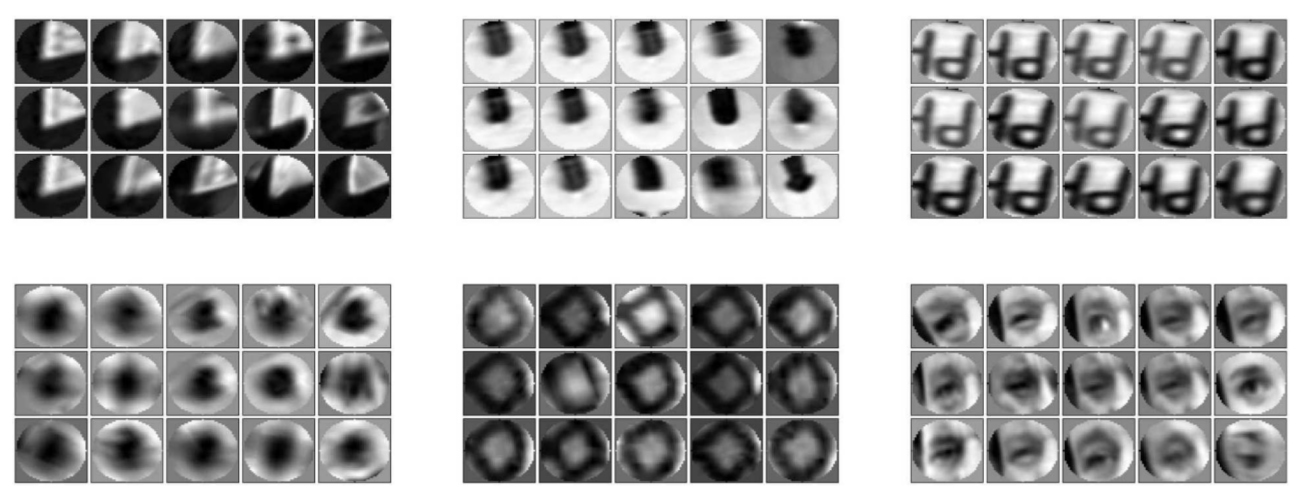
\includegraphics[scale=0.32]{visualWords}
    \else
      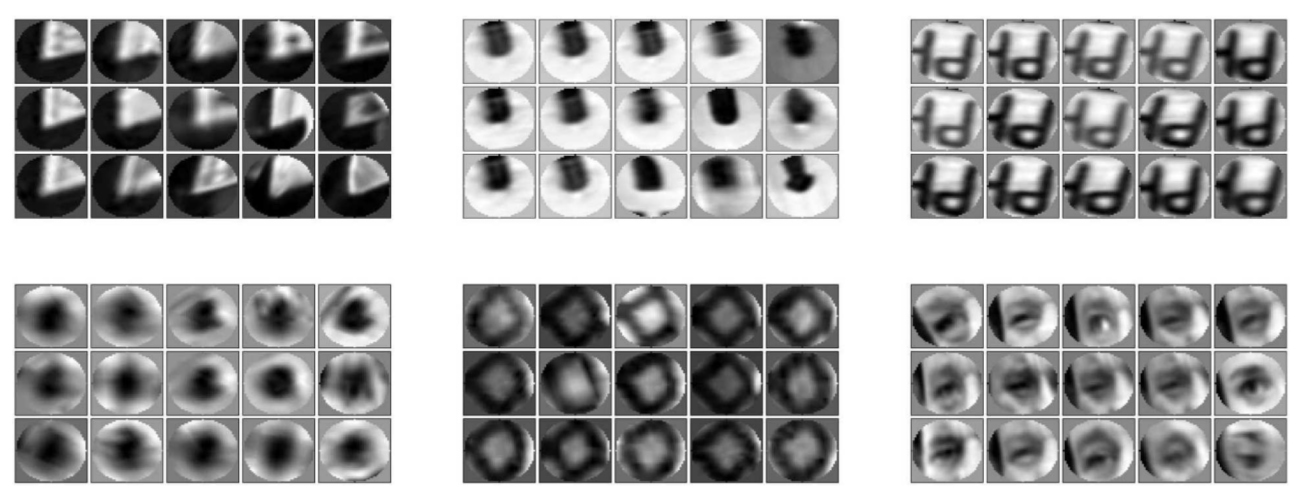
\includegraphics[scale=0.32]{visualWords}
    \fi
    \caption[Các từ trực quan (visual words)]{\textbf{Các từ trực quan (visual words).} Mỗi nhóm là một nhóm các đặc trưng cục bộ được rút trích từ hình ảnh, gom vào cùng một cụm và cùng được biểu diễn bằng một từ trực quan. Hình ảnh được lấy từ bài báo \citep{sivic2009efficient}.}
    \label{FigVisualWords}
  \end{center}
\end{figure}

Có một điều dễ thấy là nếu một hình ảnh được biểu diễn bằng càng nhiều từ trực quan thì hình ảnh đó càng "chi tiết" và độ chính xác của việc so khớp sẽ tăng lên, đồng thời nó cũng khiến cho tốc độ truy vấn nhanh hơn vì các biểu đồ bag-of-words sẽ trở nên "thưa" hơn. Trong thực tế, để truy vấn ảnh trên những tập dữ liệu lớn, để cho kết quả tốt thì số lượng từ trực quan không thể vào khoảng 10,000 từ như trong thí nghiệm của \cite{sivic2003video} mà phải lên tới hàng triệu từ. Trong khi đó, độ phức tạp của thuật toán k-means là \textit{O(N\textsubscript{w}N\textsubscript{d})} với N\textsubscript{w}, N\textsubscript{d} lần lượt là số lượng từ trực quan và số lượng "văn bản" (hình ảnh) chứa chúng. Trên những tập dữ liệu lớn thì N\textsubscript{d} $\geq$ N\textsubscript{w} nên độ phức tạp luôn lớn hơn $O(N^2_w)$. Do đó ta không thể dùng k-means cho bài toán này. \cite{nister2006scalable} đã đề xuất phương pháp giải quyết cho bài toán này bằng cách xây dựng một cây từ vựng mà về bản chất thì nó chính là thuật toán HKM (Hierarchical K-Means). Để minh họa cho thuật toán này, tác giả đã cho thử nghiệm trên bộ ảnh gồm 1 triệu hình ảnh. Không lâu sau đó, \cite{philbin2007object} đã đề xuất một hướng tiếp cận khác dựa trên thuật toán \textit{xấp xỉ k-means}, AKM (Approximate K-Means). Tác giả cũng cho chạy thử nghiệm AKM trên 16.7 triệu đặc trưng để gom cụm thành 1 triệu từ. Các thí nghiệm cho thấy rằng, khi so sánh AKM với k-means thì về độ chính xác thì AKM xấp xỉ k-means tuy nhiên chi phí tính toán chỉ bằng một phần nhỏ của k-means. Còn khi so sánh AKM với HKM thì AKM không những vượt xa về độ chính xác mà còn có thể áp dụng cho những tập dữ liệu lớn. Chi phí tính toán của cả HKM và AKM đều là $(N_d log(N_w))$.

\section{Sử dụng thông tin không gian ảnh trong truy vấn ảnh}
\label{spatial}
Mặc dù đạt được những kết quả rất đáng chú ý nhưng mô hình cơ bản của bag-of-words vẫn bị giới hạn về độ chính xác do bỏ qua một thông tin quan trọng, đó là thông tin về không gian của các đặc trưng cục bộ. Cấu trúc của mô hình bag-of-words như một cái túi chứa các từ một cách hỗn độn, không theo trật tự nên vị trí của các đặc trưng cục bộ xuất hiện trên hình không được chú ý đến, do đó các đặc trưng cục bộ được xử lý một cách rời rạc, không liên quan tới nhau. Hình \ref{FigExample} minh họa cho việc giảm độ chính xác của mô hình bag-of-words khi không chú ý tới thông tin không gian của các từ trực quan (visual words).\\ 

\begin{figure}[!htbp]
  \begin{center}
    \leavevmode
    \ifpdf
      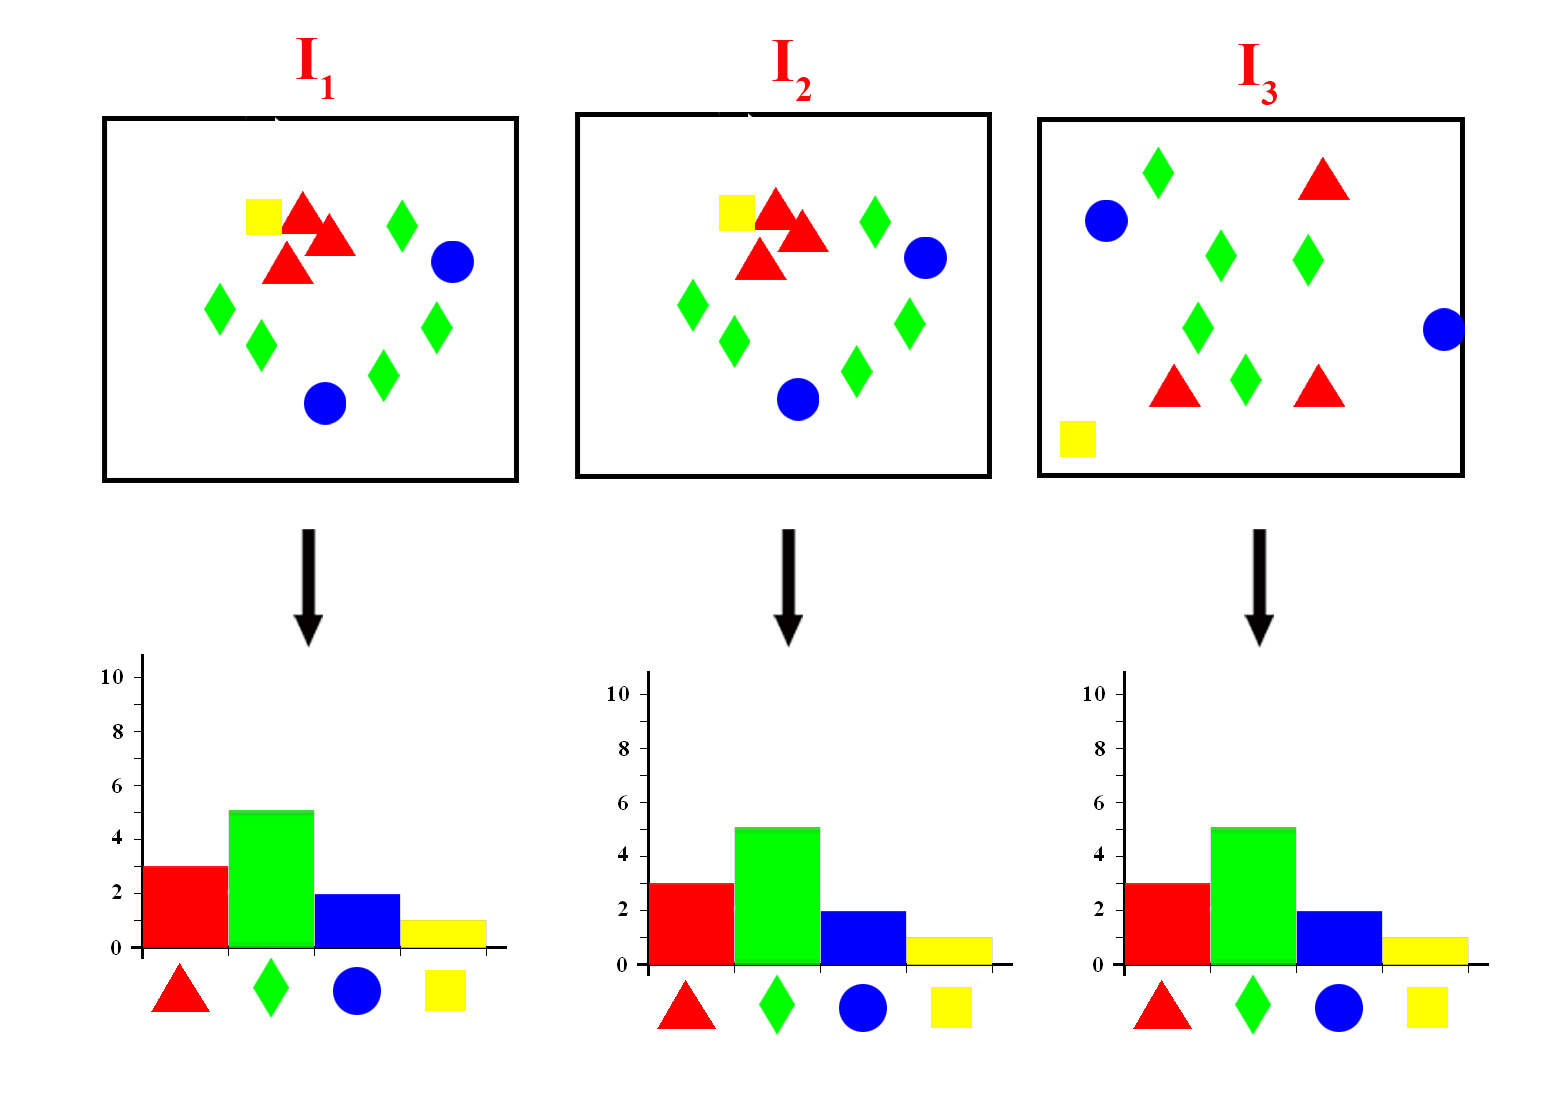
\includegraphics[scale=0.2]{example}
    \else
      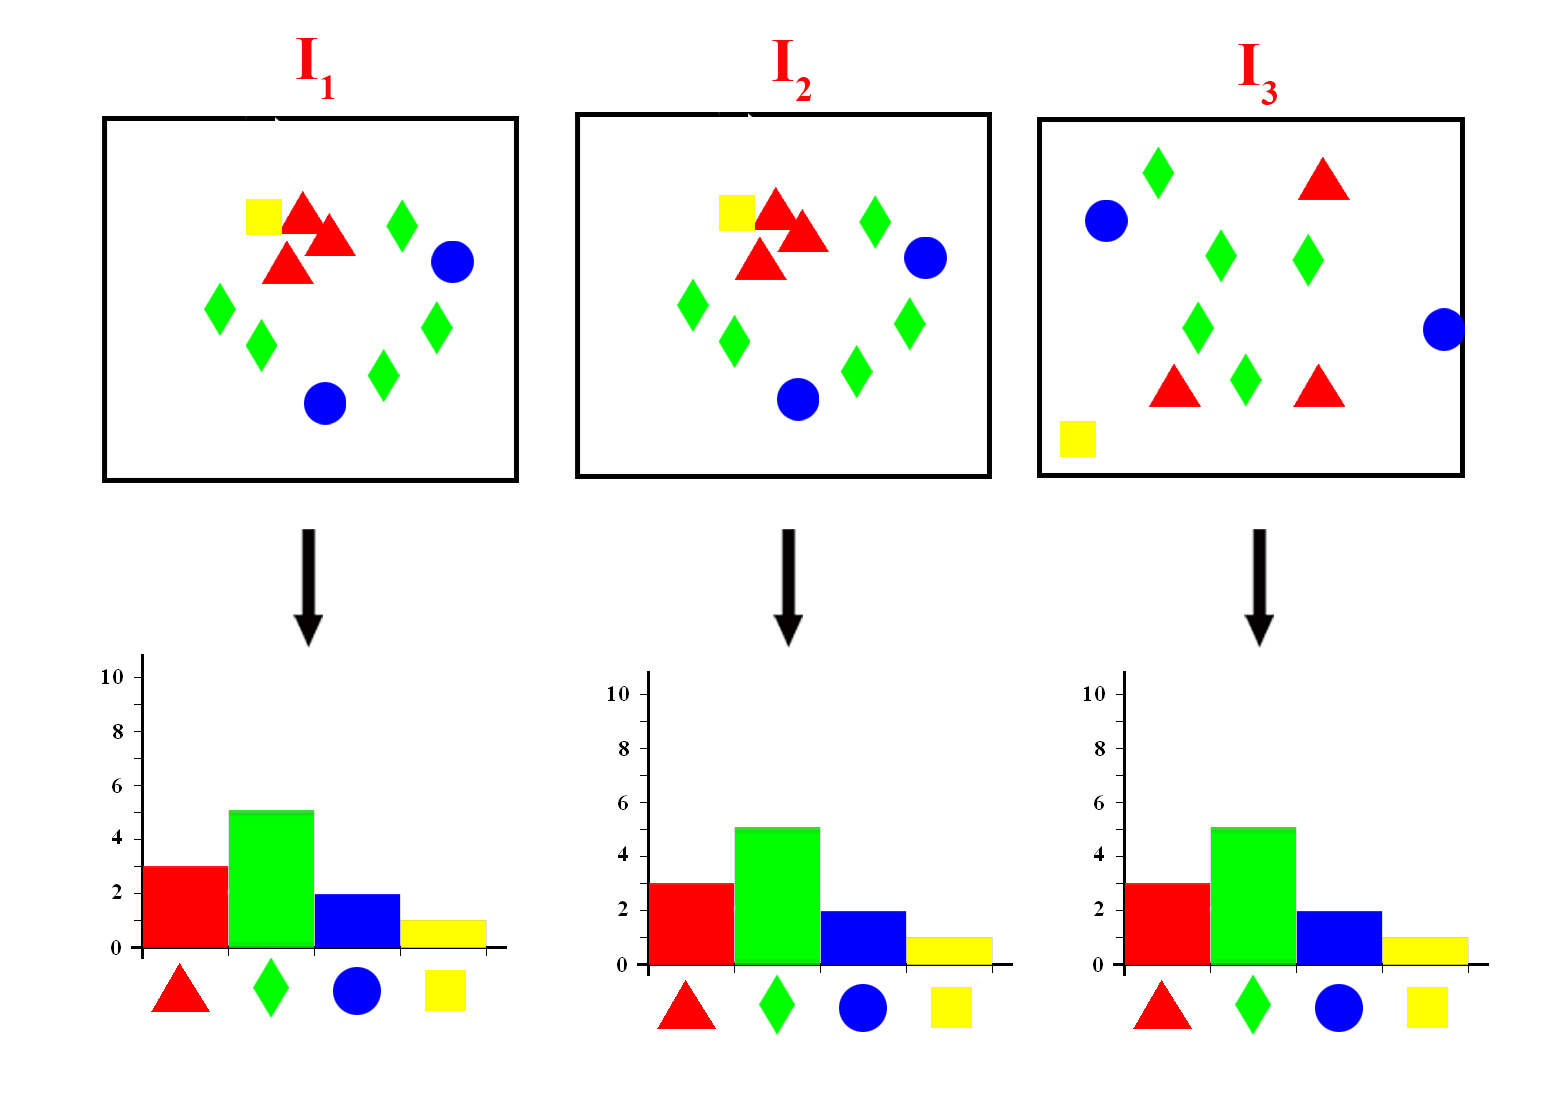
\includegraphics[scale=0.2]{example}
    \fi
    \caption[Bỏ qua thông tin không gian ảnh trong mô hình bag-of-words]{\textbf{Bỏ qua thông tin không gian ảnh trong mô hình bag-of-words.} Nếu bỏ qua thông tin không gian của các từ trực quan, ba hình ảnh trên sẽ được biểu diễn dưới dạng biểu đồ giống nhau do đó chúng sẽ được xem như ba hình ảnh giống nhau. Trong khi đó hình ảnh $I_3$ hoàn toàn khác với $I_1$ và $I_2$.}
    \label{FigExample}
  \end{center}
\end{figure}

Để giải quyết vấn đề trên, rất nhiều công trình nghiên cứu đã được đưa ra. Phần lớn các công trình nghiên cứu được chia ra làm hai dạng là tiếp cận dựa trên đặc trưng hình học và tiếp cận dựa trên thông tin không gian của các đặc trưng cục bộ. Mục \ref{geometry} chúng tôi sẽ trình bày về các phương pháp dựa trên đặc trưng hình học. Còn hướng tiếp cận còn lại sẽ được trình bày chi tiết ở mục \ref{spm}.
\subsection{Các hướng tiếp cận dựa trên đặc trưng hình học}
\label{geometry}
Các phương pháp sử dụng đặc trưng hình học để so khớp thường được dùng ở bước hậu xử lý để nhận dạng hình học. Dưới đây là một vài công trình tiêu biểu sử dụng hướng tiếp cận này.\\
\cite{sivic2003video} đã đo đạc sự nhất quán không gian cục bộ (local spatial consistency) trong các so khớp giữa hình ảnh truy vấn và từng hình ảnh trong cơ sở dữ liệu từ đó tái xếp hạng lại danh sách kết quả trả về. Việc đo đạc sự nhất quán không gian cục bộ trong so khớp hình ảnh cũng được đề cập tới trước đó trong các công trình như \cite{zhang1995robust} và \cite{schmid1997local}.\\
Trong một công trình nghiên cứu của \cite{philbin2007object}, tác giả sử dụng thuật toán RANSAC (\cite{fischler1981random}) để kiểm tra sự nhất quán hình học giữa các đặc trưng cục bộ trùng khớp. RANSAC là một trong những phương pháp phổ biến nhất cho hậu xử lý toàn cục trên hình ảnh. Đặc biệt, trong một công trình khác, \cite{zhang2011image} đề xuất mã hóa thông tin không gian ảnh qua các mệnh đề trực quan hình học (GVP) đã cho kết quả rất đáng chú ý khi kết hợp với RANSAC.\\
Trong khi đó, \cite{lin2010local} và \cite{lampert2009detecting} lại xếp hạng các hình ảnh dựa trên điểm số so khớp của hình ảnh truy vấn với những cửa sổ con được định vị trên hình. Phương pháp này mã hóa được nhiều thông tin không gian ảnh hơn so với môt hình bag-of-words trên toàn bộ tấm hình và giúp định vị hình ảnh truy vấn.\\
Nhìn chung, những phương pháp sử dụng hướng tiếp cận hình học đều cho kết quả tốt. Tuy nhiên, khi vùng truy vấn lớn hơn thì chúng chỉ được dùng để tái xếp hạng một số lượng giới hạn ở các hình ảnh ở top đầu của kết quả trả về vì vấn đề về chi phí cho bộ nhớ và tốc độ thực hiện.

\subsection{Các hướng tiếp cận dựa trên thông tin không gian của các đặc trưng cục bộ}
\label{spm}
Ut eget erat vitae odio gravida adipiscing. Pellentesque rutrum sit amet odio eget ornare. Sed non blandit ligula. Mauris mollis nibh sed eros consectetur, at semper erat dictum. Nam dolor purus, convallis a mauris aliquet, consectetur rhoncus leo. Cras nec erat eleifend, cursus purus mattis, dapibus lacus. Duis tortor nibh, consectetur eget arcu vitae, mollis laoreet magna. Vestibulum tincidunt augue ut condimentum consequat. Vestibulum vel neque mauris. Interdum et malesuada fames ac ante ipsum primis in faucibus. Nullam risus est, posuere in rhoncus a, varius non elit. Fusce a dictum eros, eget vestibulum tellus. Nunc at aliquet velit. Fusce eget quam mi. Vestibulum tristique, ligula id condimentum dapibus, nunc nisi consequat magna, vel luctus lorem quam eget velit.

Sed egestas eu lorem sollicitudin blandit. Morbi et iaculis nisi, ac consequat sem. Duis elementum leo sit amet dolor eleifend, id gravida dui mattis. Praesent malesuada, eros ac consequat auctor, ante justo lobortis dui, id malesuada lectus dolor at lorem. Phasellus ultricies rhoncus semper. Etiam lacus ligula, vehicula ut metus ac, sagittis varius quam. Nulla ut pretium tortor. Nunc feugiat, arcu et posuere consectetur, nibh diam porta eros, a consectetur leo ante ac ante. Integer malesuada laoreet augue, quis scelerisque tortor varius non. Phasellus a quam ut est tempus pharetra. Duis hendrerit eros ut lacinia tincidunt. Aenean non molestie neque. Mauris dapibus non massa eget ullamcorper. Quisque id urna vestibulum neque feugiat egestas. Praesent at egestas massa.

\section{Kết chương}
Lorem ipsum dolor sit amet, consectetur adipiscing elit. Vestibulum lectus massa, pellentesque ac rutrum sed, venenatis posuere magna. Aenean eget sagittis sem. Fusce a tortor in odio congue vehicula at condimentum urna. Suspendisse nec tortor nec tortor rutrum laoreet vitae nec lacus. Quisque sed purus vitae ipsum porta malesuada. Nullam sed turpis vitae nulla fringilla ullamcorper. Aenean vitae ligula enim. Suspendisse eu molestie nulla. Praesent id lacus tincidunt, lacinia eros sit amet, sagittis urna. Etiam nisl purus, varius non quam vel, pretium tincidunt est. Aliquam erat volutpat. Fusce auctor mattis neque, ut ultrices nisl gravida at. Etiam vel placerat erat. Donec rutrum viverra lacus sit amet gravida. Fusce vel nibh a risus condimentum feugiat eget vitae enim. Curabitur sem sem, convallis vitae consectetur id, condimentum sit amet libero.

